% !Mode:: "TeX:UTF-8"
\documentclass[arialtitle=false,type=doctor]{plutothesis}

\usepackage{lipsum}
\graphicspath{{figures/}}

\begin{document}
\frontmatter
% !Mode:: "TeX:UTF-8" 

\newcommand{\chinesethesistitle}{局部多孔质气体静压轴承关键技术的研究} %授权书用,无需断行
\newcommand{\englishthesistitle}{\uppercase{RESEARCH ON KEY TECHNOLOGIES OF PARTIAL POROUS EXTERNALLY PRESSURIZED GAS BEARING}} %\uppercase作用:将英文标题字母全部大写;
\newcommand{\chinesethesistime}{2010 年~12 月}  %封面底部的日期中文形式
\newcommand{\englishthesistime}{December, 2010}    %封面底部的日期英文形式

\ctitle{局部多孔质气体静压轴承关键技术的研究}  %封面用论文标题,自己可手动断行
\cdegree{\cxueke\cxuewei}
\csubject{机械制造及其自动化}                 %(~按二级学科填写~)
\caffil{机电工程学院} %(在校生填所在系名称,同等学力人员填工作单位)
\cauthor{于冬梅}
\csupervisor{某某某教授} %导师名字
\cassosupervisor{副导名}%若没有,请屏蔽掉此句。
\ccosupervisor{联导名}%若没有,请屏蔽掉此句。


\cdate{\chinesethesistime}

\etitle{\englishthesistitle}
\edegree{\exuewei \ of \exueke}
\esubject{Mechanical Manufacturing and Automation}  %英文二级学科名
\eaffil{School of Mechatronics Engineering}
\eauthor{Yu Dongmei}                   %作者姓名 (英文)
\esupervisor{Prof. XXX}       % 导师姓名 (英文)
\eassosupervisor{Prof. Assosuper}%若没有,请屏蔽掉此句。
\ecosupervisor{Prof. Cosuper}%若没有,请屏蔽掉此句。
\edate{\englishthesistime}

\natclassifiedindex{TM301.2}  %国内图书分类号
\internatclassifiedindex{62-5}  %国际图书分类号
\statesecrets{公开} %秘密

\iffalse
\BiAppendixChapter{摘~~~~要}{}
\fi
\cabstract{
摘要是论文内容的高度概括,应具有独立性和自含性,即不阅读论文的全文,就能获得必要的信息。
摘要应包括本论文的目的、主要研究内容、研究方法、创造性成果及其理论与实际意义。
摘要中不宜使用公式、化学结构式、图表和非公知公用的符号和术语,不标注引用文献编号。避免将摘要写成目录式的内容介绍。
}

\ckeywords{关键词~1;关键词~2;关键词~3;……;关键词~6(关键词总共~3~—~6~个,最后一个关键词后面没有标点符号)}

\eabstract{
Externally pressurized gas bearing has been widely used in the field of aviation, semiconductor, weave, and measurement apparatus because of its advantage of high accuracy, little friction, low heat distortion, long life-span, and no pollution. In this thesis, based on the domestic and overseas researching……

}

\ekeywords{keyword 1, keyword 2, keyword 3, ……, keyword 6 (no punctuation at the end) 英文摘要与中文摘要的内容应一致,在语法、用词上应准确无误。}

\makecover
\clearpage 
 % 封面
\makecover

\pdfbookmark[0]{目~录}{mulu}
\tableofcontents    % 中文目录
\tableofengcontents % 英文目录
\mainmatter

\layout

% !Mode:: "TeX:UTF-8" 

\BiChapter{图片的插入方法}{Methods of inserting figures}

\BiSection{研究生院的插图规范}{Figures inserting standard from graduate school}
图应有自明性。插图应与文字紧密配合,文图相符,内容正确。选图要力求精练,插图、照片应完整清晰。图中文字和数字等字号用宋体~5~号字。

机械工程图:采用第一角投影法,严格按照~GB4457---GB131-83《机械制图》标准规定。

数据流程图、程序流程图、系统流程图等按~GB1526-89~标准规定。

电气图:图形符号、文字符号等应符合附录~3~所列有关标准的规定。

流程图:必须采用结构化程序并正确运用流程框图。

对无规定符号的图形应采用该行业的常用画法。

坐标图的坐标线均用细实线,粗细不得超过图中曲线,有数字标注的坐标图,必须注明坐标单位。

照片图要求主题和主要显示部分的轮廓鲜明,便于制版。如用放大或缩小的复制品,必须清晰,反差适中。照片上应有表示目的物尺寸的标度。

引用文献图表必须标注出处。


\BiSubsection{图题及图中说明}{Captions and descriptions of figures}
每个图均应有图题(由图序和图名组成),图名在图序之后空一格排写。图序按章编排,如第~1~章第一个插图的图号为“图~1-1”等。
图题置于图下,硕士论文可只用中文书写,博士论文用中、英文两种文字居中书写,中文在上,要求中文用宋体~5~号字,英文用~Times New Roman 5~号字。有图注或其它说明时应置于图题之上。引用图应注明出处,在图题右上角加引用文献号。
图中若有分图时,分图题置于分图之下或图题之下,分图号用~a)、b)等表示。

图中各部分说明应采用中文(引用的外文图除外)或数字项号,各项文字说明置于图题之上(有分图题者,置于分图题之上)。

\BiSubsection{插图编排}{Layouts of illustrations}
插图之前,文中必须有关于本插图的提示,如“见图~1-1”、“如图~1-1~所示”等。插图与其图题为一个整体,不得拆开排写于两页。
插图处的该页空白不够排写该图整体时,则可将其后文字部分提前排写,将图移到次页。

\BiSection{\LaTeX~中推荐使用的图片格式}{Recommended figure format applied in \LaTeX}
在~\LaTeX~中应用最多的图片格式是~EPS(Encapsulated PostScript)格式,它是一种专用的打印机描述语言,常用于印刷或打印输出。
EPS~格式图片可通过多种方式生成,这里介绍一款功能强大的免费图片处理软件———\href{http://www.imagemagick.org/}{ImageMagick},
360~软件管家也提供此软件的下载。此软件可将其它格式图片转换为~EPS~格式图片,同时还可以锐化图片,使图片的局部清晰一些。

此软件对图片的格式转换操作都是在命令提示符(cmd.exe)中实现的,可以通过“开始$\to$运行$\to$输入~cmd$\to$回车”或
“开始$\to$程序$\to$附件$\to$命令提示符”找到它。在命令提示符下,首先采用“盘符命令”或“cd~命令”将当前目录改为待处理图片所在的目录,
在此目录下就可通过~convert~命令将图片转换为~EPS~格式,其命令的语法格式为

\noindent\verb|convert [可选参数] 原文件名.原扩展名 新文件名.eps|

\noindent 若~convert~命令中无可选参数,则将原来的图片格式直接转换为~EPS~格式,对图片不进行任何处理,这也是最常用的方法。
也可以选用可选参数,可选参数有很多选择,但最常用的有如下两个:

\verb|-sharpen radius{xsigma}|———此参数用来锐化图片,一般用在图片像素不高,需要提高图片清晰度的情况下。其中~radius~只能为整数,
它用来确定转换命令采取哪一种锐化算法,我们可以只取~radius~为~0;sigma~为所采取算法的锐化度,它的取值为~0.1--3~之间的任意一个浮点数,
数值越大,锐化程度也越大,通常取为~0.5--1~之间;x在参数中为分隔符。

\verb|-resize geometry|———此参数用来改变图片的大小,若图片的存储空间过大,可通过此命令缩小图片尺寸,但同时也将导致图片像素降低,
其具体用法请参见\href{http://www.imagemagick.org/script/command-line-options.php#resize}{-resize geometry的官方说明}。

除此之外,一些文字处理软件和科学计算软件也支持生成~EPS~格式的文件,请使用“另存为”功能查看某款软件是否能够将图片以~EPS~格式的形式保存。

\BiSection{单张图片的插入方法}{The method of inserting one single figure}
单张图片独自占一行的插入形式如图~\ref{golfer1}~所示。
\begin{figure}[htbp]
\centering
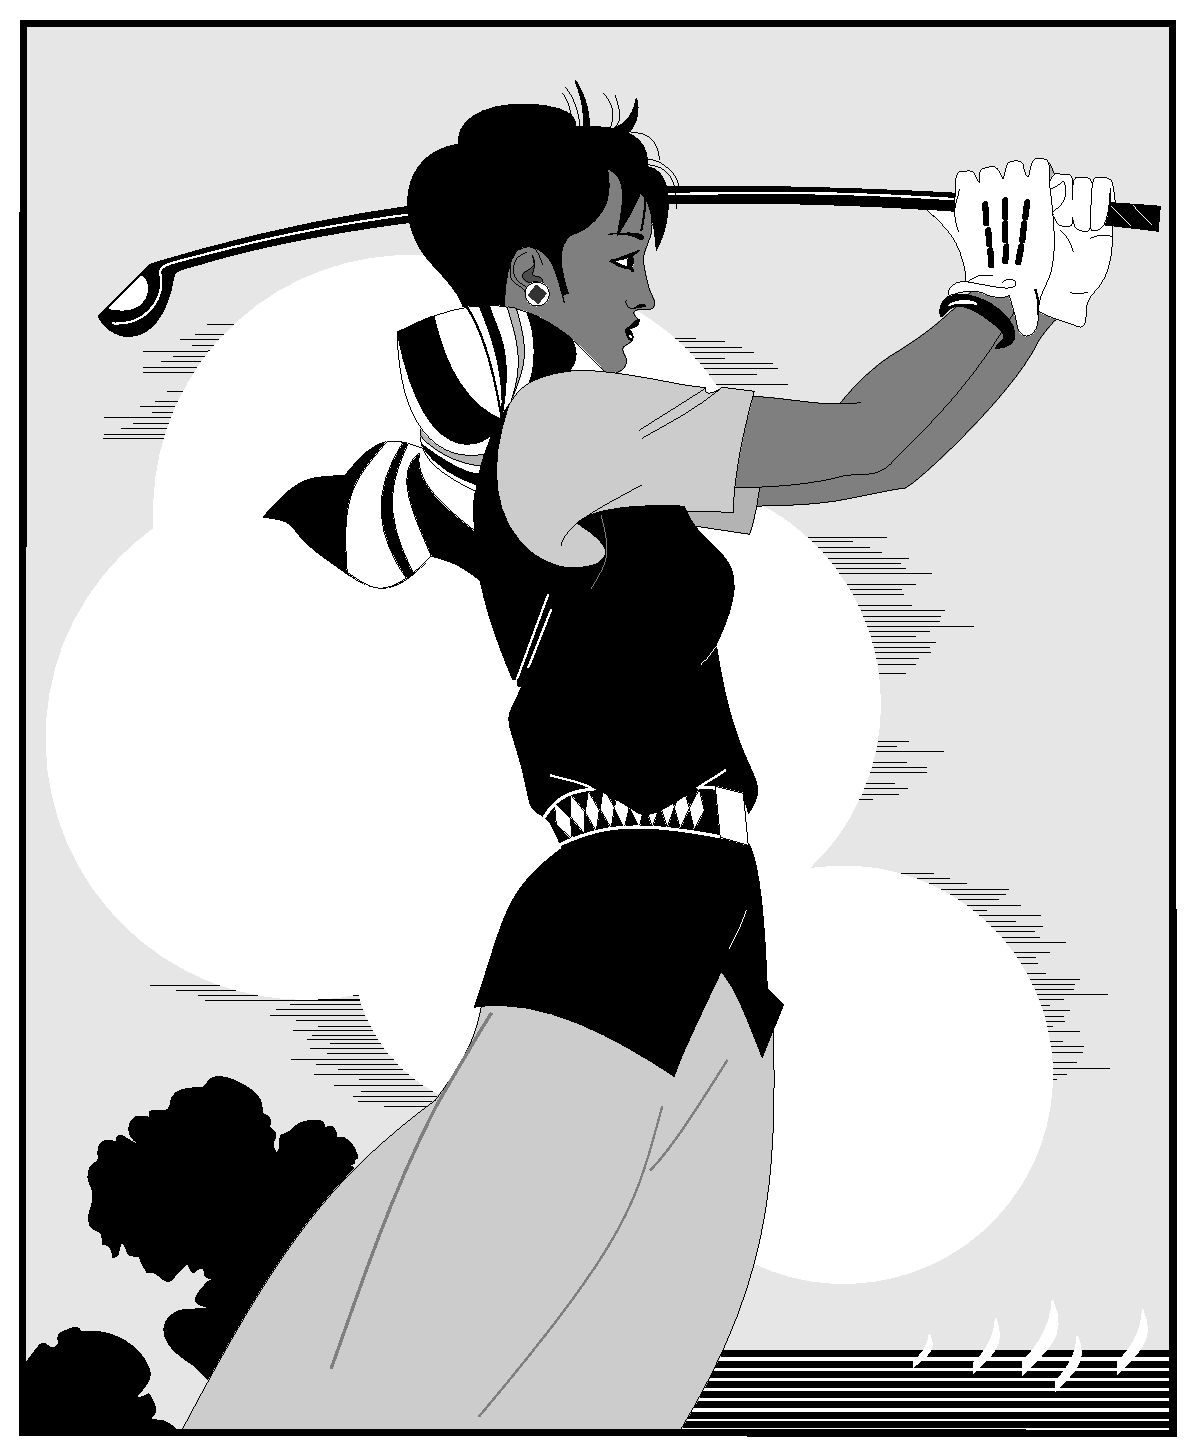
\includegraphics[width = 0.4\textwidth]{golfer}
\bicaption[golfer1]{}{打高尔夫球的人}{Fig.$\!$}{The person playing golf}\vspace{-1em}
\end{figure}

其插入图片的代码及其说明如下。
\vspace{1em}\noindent\hrule
\begin{verbatim}
\begin{figure}[htbp]
\centering
\includegraphics[width=0.4\textwidth]{文件名(.eps)}
\bicaption[标签名(英文)]{}{中文标题}{Fig.$\!$}
          {English caption (首字母大写)}\vspace{-1em}
\end{figure}
\end{verbatim}
\noindent\hrule
\begin{verbatim}
figure环境的可选参数[htbp]表示浮动图形所放置的位置,h (here)表示当前位置,t (top)表示页芯顶部,b (bottom)表示页芯底部,p (page)表示单独一页。在word等软件中,图片通常插入到当前位置,如果当前页的剩余空间不够,图片将被移动到下一页,当前页就会出现很大的空白,其人工调整工作非常不便。由LaTeX提供的浮动图片功能,总是会按h->t->b->p的次序处理选项中的字母,自动调整图片的位置,大大减轻了工作量。
\centering命令将后续内容转换成每行皆居中的格式。
“\includegraphics”的可选参数用来设置图片插入文中的水平宽度,一般表示为正文宽度(\textwidth)的倍数。
\bicaption命令的使用需要调用ccaption宏包,它可以为图片或表格插入双语标题(博士学位论文要求),可选参数“标签名”为英文形式,一般不以图片或表格的数字顺序作为标签,而应包含一定的图片或表格信息,以便于文中引用(若图片、表格、公式、章节和参考文献等在文中出现的先后顺序发生了变化,其标注序号及其文中引用序号也会跟着发生变化,这一点是word等软件所不能做到的)。第4个参数中的“$\!$”表示-1/6个空铅宽度,这样可以缩小Fig.和Table与后面数字序号之间的水平距离。另外,图题或表题并不会因为分页而与图片或表格体分置于两页,章节等各级标题也不会置于某页的最底部,LaTeX系统会自动调整它们在正文中的位置,这也是word等软件所无法匹敌的。
注:硕士学位论文的图表只需要插入中文标题,因此需将\bicaption一句命令替换为如下两条命令(下同):
\caption{中文标题}
\label{标签名(英文)}
\vspace将产生一定高度的竖直空白,必选参数为负值表示将后续文字位置向上提升,参数值可自行调整。em为长度单位,相当于大写字母M的宽度。
引用方法:“见图~\ref{标签名(英文)}”、“如图~\ref{标签名(英文)}~所示”等。
\end{verbatim}
\noindent\hrule\vspace{1em}
若需要将~2~张及以上的图片并排插入到一行中,则需要采用\verb|minipage|环境,如图~\ref{golfer2}~和图~\ref{golfer3}~所示。
\begin{figure}[htbp]
\centering
\begin{minipage}{0.4\textwidth}
\centering
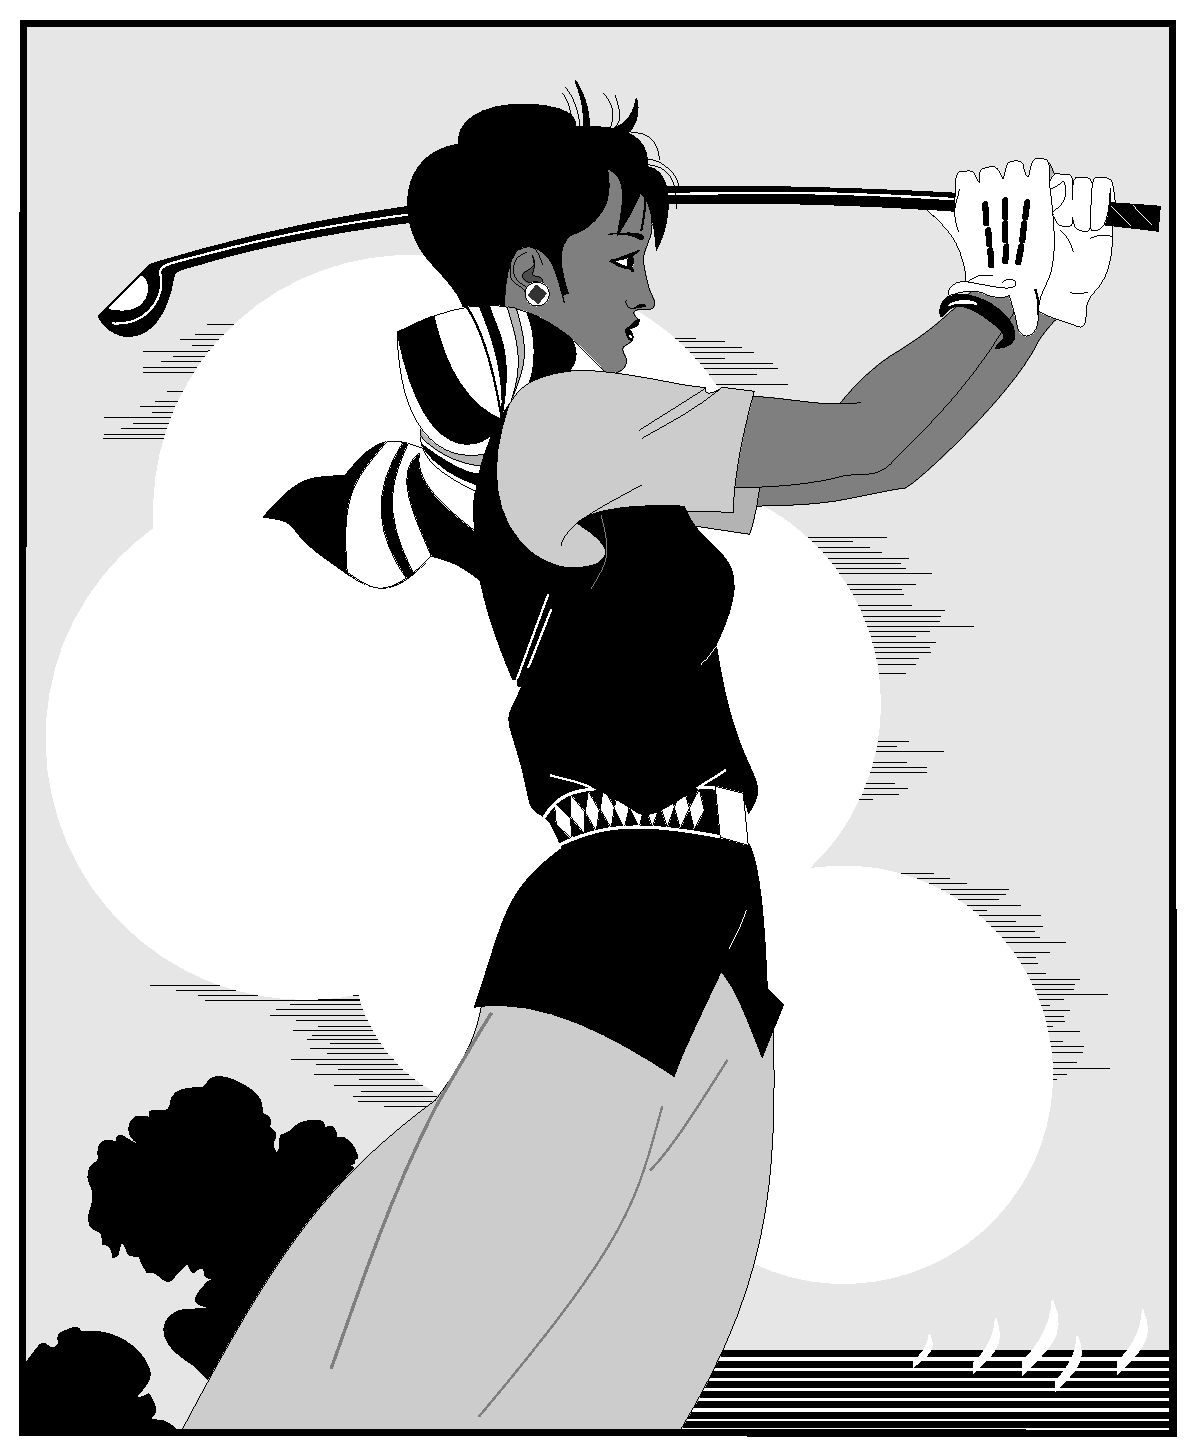
\includegraphics[width=\textwidth]{golfer}
\bicaption[golfer2]{}{打高尔夫球的人}{Fig.$\!$}{The person playing golf}
\end{minipage}
\begin{minipage}{0.4\textwidth}
\centering
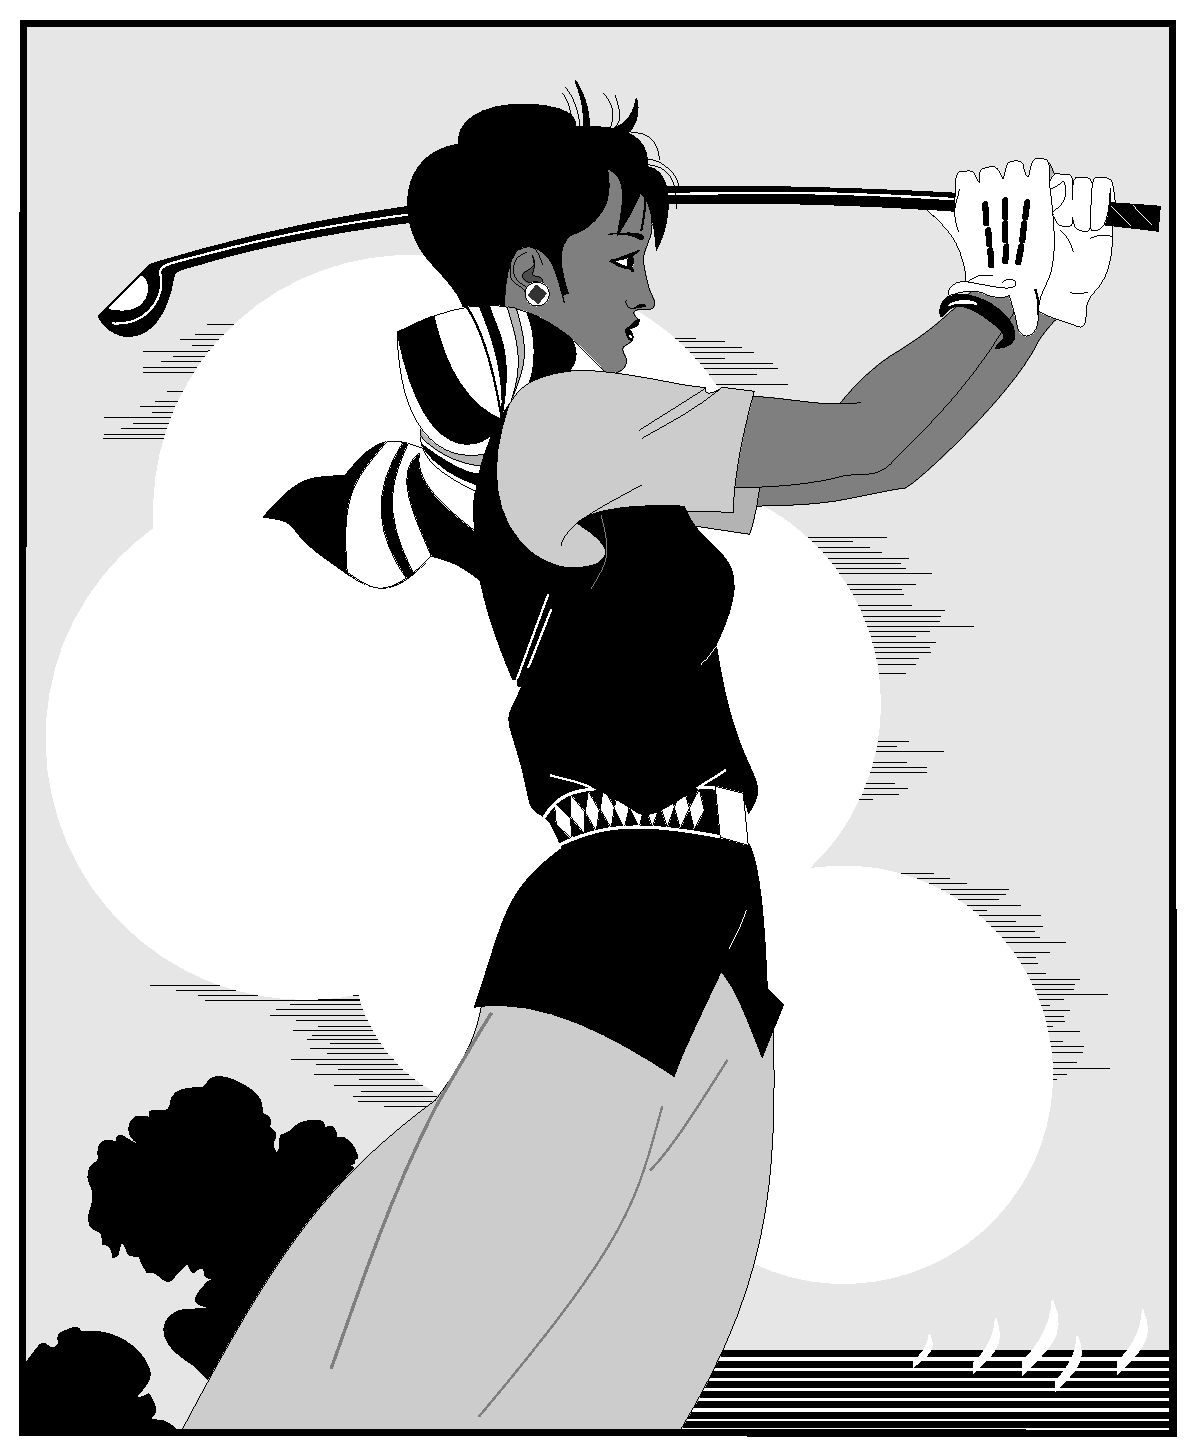
\includegraphics[width=\textwidth]{golfer}
\bicaption[golfer3]{}{打高尔夫球的人}{Fig.$\!$}{The person playing golf}
\end{minipage}\vspace{-1em}
\end{figure}

其代码如下所示。
\vspace{1em}\noindent\hrule
\begin{verbatim}
\begin{figure}[htbp]
\centering
\begin{minipage}{0.4\textwidth}
\centering
\includegraphics[width=\textwidth]{文件名}
\bicaption[标签名]{}{中文标题}{Fig.$\!$}
          {English caption}
\end{minipage}
\begin{minipage}{0.4\textwidth}
\centering
\includegraphics[width=\textwidth]{文件名}
\bicaption[标签名]{}{中文标题}{Fig.$\!$}
          {English caption}
\end{minipage}\vspace{-1em}
\end{figure}
\end{verbatim}
\noindent\hrule
\begin{verbatim}
minipage环境的必选参数用来设置小页的宽度,若需要在一行中插入n个等宽图片,则每个小页的宽度应略小于(1/n)\textwidth。
\end{verbatim}
\noindent\hrule

\BiSection{具有子图的图片插入方法}{The method of inserting figures with subfigures}

图中若含有子图时,需要调用~subfigure~宏包。博士学位论文规范要求不止总图的标题为中英文形式,其各个子图也应具有中英文形式的标题。
然而~ccaption~宏包却无法实现子图的中英文标题功能,这里采用对\verb|\subfigure|命令进行嵌套的方法来实现子图的中英文标题功能,如图~\ref{golfer4}~所示。

\begin{figure}[htbp]
\centering
\subfigure{\label{golfer41}}\addtocounter{subfigure}{-2}
\subfigure[The person playing golf]{\subfigure[打高尔夫球的人~1]{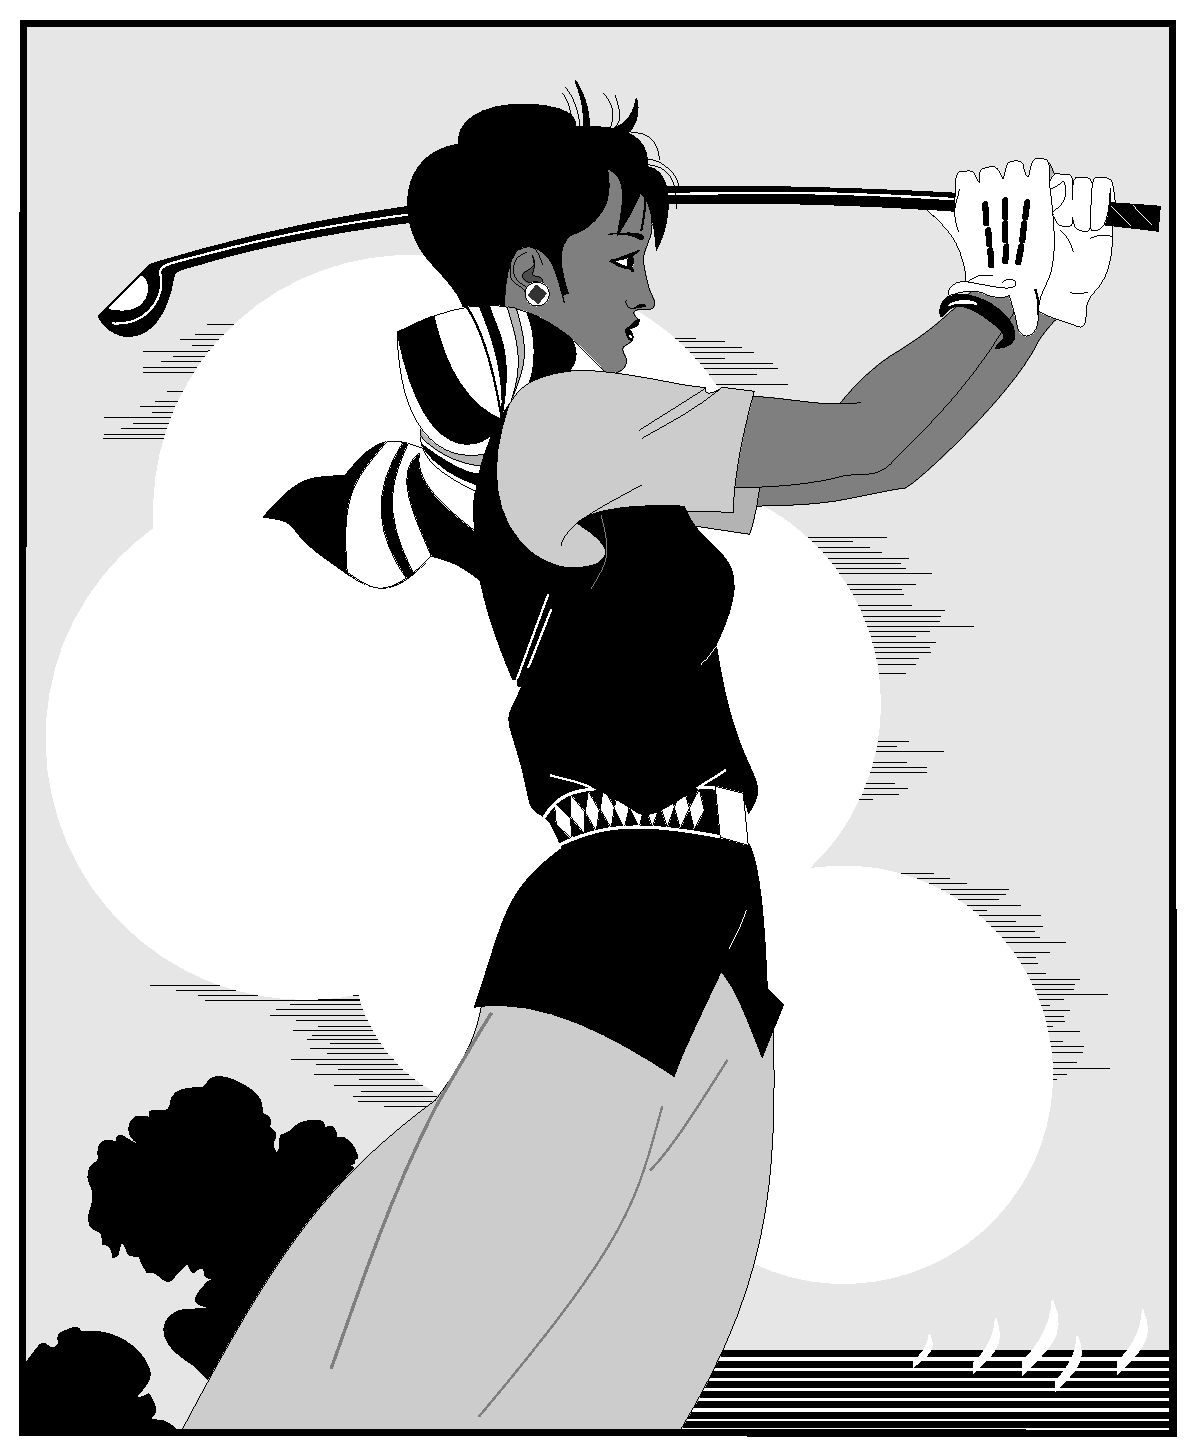
\includegraphics[width=0.4\textwidth]{golfer}}}
\subfigure{\label{golfer42}}\addtocounter{subfigure}{-2}
\subfigure[The person playing golf]{\subfigure[打高尔夫球的人~2]{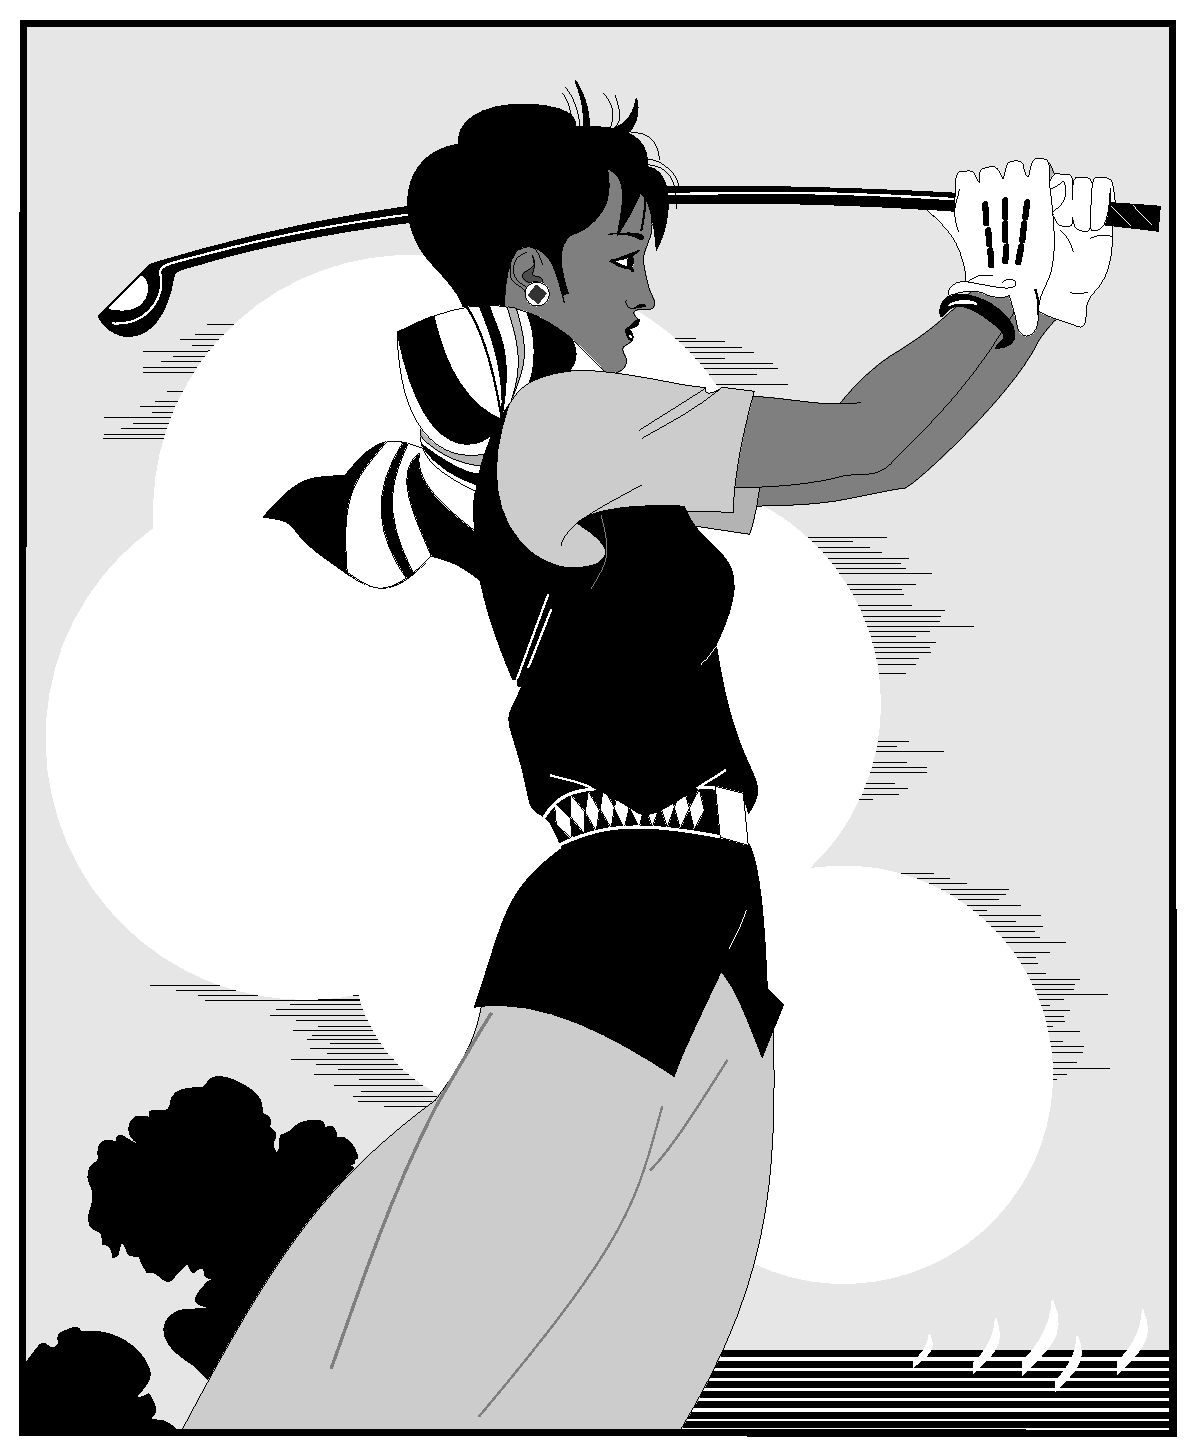
\includegraphics[width=0.4\textwidth]{golfer}}}
\bicaption[golfer4]{}{打高尔夫球的人}{Fig.$\!$}{The person playing golf}\vspace{-1em}
\end{figure}

其代码及其说明如下。
\vspace{1em}\noindent\hrule
\begin{verbatim}
\begin{figure}[htbp]
\centering
\subfigure{\label{第1个子图标签名}}\addtocounter{subfigure}{-2}
\subfigure[The 1st subfigure caption]{\subfigure[第1个子图标题]
          {\includegraphics[width=0.4\textwidth]{文件名}}}
\subfigure{\label{第2个子图标签名}}\addtocounter{subfigure}{-2}
\subfigure[The 2nd subfigure caption]{\subfigure[第2个子图标题]
          {\includegraphics[width=0.4\textwidth]{文件名}}}
\bicaption[总标签名]{}{中文总标题}{Fig.$\!$}{The total caption}
\vspace{-1em}
\end{figure}
\end{verbatim}
\noindent\hrule
\begin{verbatim}
\addtocounter把指定的值加到计数器上,这里是对subfigure计数器进行减2操作。这是因为每插入1个子图,就调用3次\subfigure命令,第1次调用\subfigure命令用来生成紧随其后所插入子图的标签,而之后的双层嵌套调用\subfigure命令用来插入子图并生成该子图的中英文标题。因此,每插入1张子图,subfigure计数器的值就自动加3,为了使得子图的序号能每次加1,则需在每插入1张子图前手动把subfigure计数器的值减2。
\subfigure命令的双层嵌套使用可用来生成中英文标题,其内层\subfigure命令用来插入子图并生成中文标题,外层\subfigure命令将插入的子图和中文标题作为一个整体,生成这个整体的英文标题,因此英文标题会置于中文标题的下面。
硕士学位论文只需要中文标题,其代码如下:
\begin{figure}[htbp]
\centering
\subfigure[第1个子图标题\label{第1个子图标签名}]
          {\includegraphics[width=0.4\textwidth]{文件名}}
\subfigure[第2个子图标题\label{第2个子图标签名}]
          {\includegraphics[width=0.4\textwidth]{文件名}}
\caption{中文总标题}\label{总标签名}
\vspace{-1em}
\end{figure}
引用方法:总图的引用方法同本章第1节,子图的引用方法用\ref{第n个子图标签名}来代替。
\end{verbatim}
\noindent\hrule\vspace{1em}

子图的引用示例:如图~\ref{golfer41}~和图~\ref{golfer42}~所示。

若想获得插图方法的更多信息,请参见网络上的~\href{ftp://ftp.tex.ac.uk/tex-archive/info/epslatex.pdf}{Using Imported Graphics in \LaTeX and pdf\LaTeX}~文档。  % 封面

\bibliographystyle{GBT7714-2005NLang-HIT}
\addcontentsline{toc}{chapter}{参考文献}      % 参考文献加入到中文目录
\addcontentsline{toe}{chapter}{\bfseries  References} % 参考文献加入到英文目录
\addtolength{\bibsep}{-0.8em}
%\nocite{*}  %若将此命令屏蔽掉,则未引用的文献不会出现在文后的参考文献列表中。
\bibliography{reference}
%\renewcommand{\appendixname}{附录~\Alph{chapter}}
%\renewcommand{\theequation}{\Alph{chapter}-\arabic{equation}}
%\renewcommand{\thetable}{\Alph{chapter}-\arabic{table}}
%% -*-coding: utf-8 -*-

\defaultfont
\appendix

%%%%%%%%%%%%%%%%%%%%%%%%%%%%%%%%%%%%%%%%%%%%%%%%%%%%%%%%%
\BiAppChapter{带章节的附录}{Full Appendix}%
完整的附录内容,包含章节,公式,图表等

%%%%%%%%%%%%%%%%%%%%%%%%%%%%%%%%%%%%%%%%%%%%%%%%%%%%%%%%%
\BiSection{附录节的内容}{Section in Appendix}
这是附录的节的内容

附录中图的示例:
\begin{figure}[htbp]
\centering
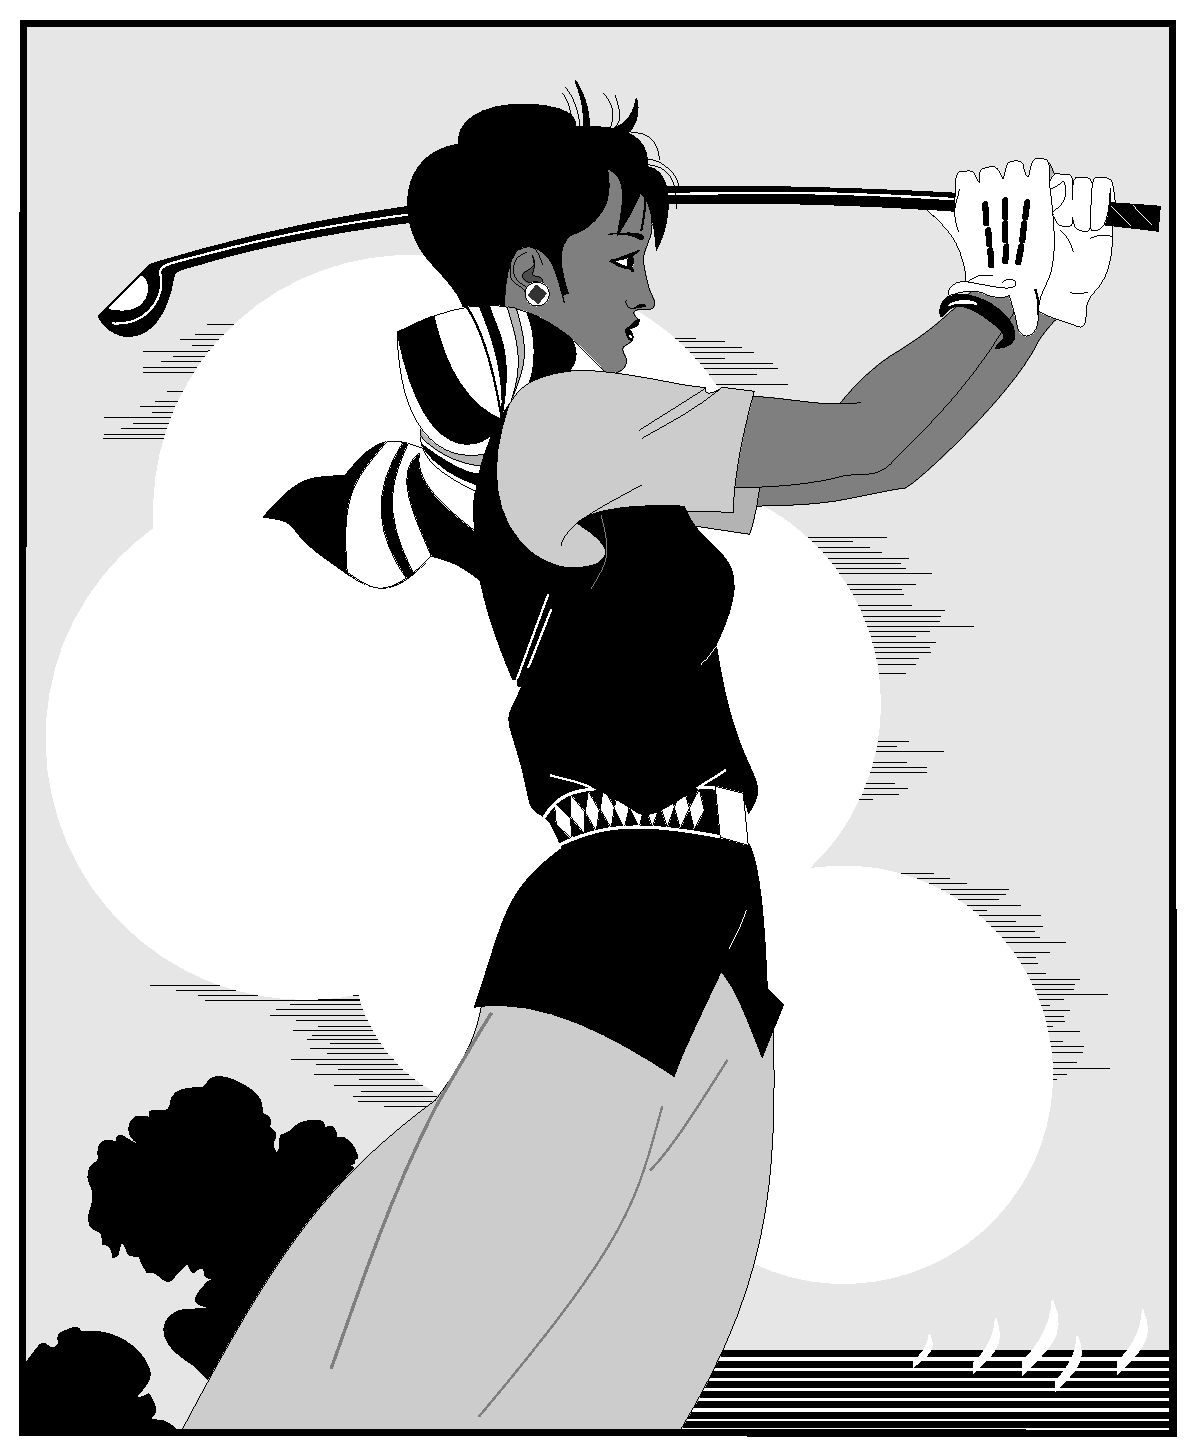
\includegraphics[width = 0.4\textwidth]{golfer}
\bicaption[golfer5]{}{打高尔夫球的人}{Fig.$\!$}{The person playing golf}\vspace{-1em}
\end{figure}

附录中公式的示例:
\begin{align}
a & = b \times c \\
E & = m c^2
\end{align}

\BiAppChapter{这个星球上最好的免费Windows软件列表}{List of the Best Free Windows Software in our Planet}
\section*{杀毒软件}
\href{http://www.avast.com/zh-cn/free-antivirus-download}{avast! 免费杀毒软件}——推荐

\href{http://www.avg.com/cn-zh/china-avg-antivirus-free}{AVG 杀毒永久免费版}——推荐

\href{http://www.avira.com/en/avira-free-antivirus}{Avira Free Antivirus (小红伞)}









%\BiAppChapter{附录三}{appendix 3}    % 附录
%% !Mode:: "TeX:UTF-8" 

\BiAppendixChapter{攻读\cxuewei 学位期间发表的论文及其他成果} {Papers
published in the period of PH.D. education}
\noindent\textbf\song{(一)发表的学术论文}
\begin{publist}
\item	XXX,XXX. Static Oxidation Model of Al-Mg/C Dissipation Thermal Protection Materials[J]. Rare Metal Materials and Engineering, 2010, 39(Suppl. 1): 520-524.(SCI~收录,IDS号为~669JS,IF=0.16)
\item XXX,XXX. 精密超声振动切削单晶铜的计算机仿真研究[J]. 系统仿真学报,2007,19(4):738-741,753.(EI~收录号:20071310514841)
\item XXX,XXX. 局部多孔质气体静压轴向轴承静态特性的数值求解[J]. 摩擦学学报,2007(1):68-72.(EI~收录号:20071510544816)
\item XXX,XXX. 硬脆光学晶体材料超精密切削理论研究综述[J]. 机械工程学报,2003,39(8):15-22.(EI~收录号:2004088028875)
\item XXX,XXX. 基于遗传算法的超精密切削加工表面粗糙度预测模型的参数辨识以及切削参数优化[J]. 机械工程学报,2005,41(11):158-162.(EI~收录号:2006039650087)
\item XXX,XXX. Discrete Sliding Mode Cintrok with Fuzzy Adaptive Reaching Law on 6-PEES Parallel Robot[C]. Intelligent System Design and Applications, Jinan, 2006: 649-652.(EI~收录号:20073210746529)
\end{publist}

\noindent\textbf\song{(二)申请及已获得的专利(无专利时此项不必列出)}
\begin{publist}
\item XXX,XXX. 一种温热外敷药制备方案:中国,88105607.3[P]. 1989-07-26.
\end{publist}

\noindent\textbf\song{(三)参与的科研项目及获奖情况}
\begin{publist}
\item	XXX,XXX. XX~气体静压轴承技术研究, XX~省自然科学基金项目.课题编号:XXXX.
\item XXX,XXX. XX~静载下预应力混凝土房屋结构设计统一理论. 黑江省科学技术二等奖, 2007.
\end{publist}
%\vfill
%\hangafter=1\hangindent=2em\noindent

%\setlength{\parindent}{2em}
    % 所发文章
%% !Mode:: "TeX:UTF-8" 

\BiAppendixChapter{哈尔滨工业大学学位论文原创性声明和使用权限}{Statement of copyright and Letter of authorization}
\vspace{\baselineskip}
\begin{center}\hei\xiaosan{学位论文原创性声明}\end{center}
\vspace{1em}

本人郑重声明:此处所提交的学位论文《\chinesethesistitle》,是本人在导师指导下,在哈尔滨工业大学攻读学位期间独立进行研究工作所取得的成果,且学位论文中除已标注引用文献的部分外不包含他人完成或已发表的研究成果。对本学位论文的研究工作做出重要贡献的个人和集体,均已在文中以明确方式注明。

\vspace{\baselineskip}
\hspace{6em}作者签名:\hfill 日期:\hspace{2.5em}年\hspace{1.5em}月\hspace{1.5em}日

\vspace{2\baselineskip}
\begin{center}\hei\xiaosan{学位论文使用权限}\end{center}
\vspace{1em}

学位论文是研究生在哈尔滨工业大学攻读学位期间完成的成果,知识产权归属哈尔滨工业大学。学位论文的使用权限如下:

(1)学校可以采用影印、缩印或其他复制手段保存研究生上交的学位论文,并向国家图书馆报送学位论文;(2)学校可以将学位论文部分或全部内容编入有关数据库进行检索和提供相应阅览服务;(3)研究生毕业后发表与此学位论文研究成果相关的学术论文和其他成果时,应征得导师同意,且第一署名单位为哈尔滨工业大学。

保密论文在保密期内遵守有关保密规定,解密后适用于此使用权限规定。

本人知悉学位论文的使用权限,并将遵守有关规定。


\vspace{2\baselineskip}
\hspace{6em}作者签名:\hfill 日期:\hspace{2.5em}年\hspace{1.5em}月\hspace{1.5em}日

\vspace{2\baselineskip}
\hspace{6em}导师签名:\hfill 日期:\hspace{2.5em}年\hspace{1.5em}月\hspace{1.5em}日   % 承诺
%% !Mode:: "TeX:UTF-8" 

\BiAppendixChapter{致\quad 谢}{Acknowledgements}

衷心感谢导师~XXX~教授对本人的精心指导。他的言传身教将使我终生受益。

感谢~XXX~教授,以及实验室全体老师和同窗们的热情帮助和支持!

本课题承蒙~XXXX~基金资助,特此致谢。

…
% 致谢
%\ifxueweidoctor
%% !Mode:: "TeX:UTF-8" 

\defaultfont

\BiAppendixChapter{个人简历}{Resume}

XXXX~年~XX~月~XX~日出生于~XXXX。

XXXX~年~XX~月考入~XX~大学~XX~院(系)XX~专业,XXXX~年~XX~月本科毕业并获得~XX~学学士学位。

XXXX~年~XX~月------XXXX~年~XX~月在~XX~大学~XX~院(系)XX~学科学习并获得~XX~学硕士学位。

XXXX~年~XX~月------XXXX~年~XX~月在~XX~大学~XX~院(系)XX~学科学习并获得~XX~学博士学位。

获奖情况:如获三好学生、优秀团干部、X~奖学金等(不含科研学术获奖)。

工作经历:

\vspace{3em}\noindent
\textbf{( 除全日制硕士生以外,其余学生均应增列此项。个人简历一般应包含教育经历和工作经历。)}          % 博士学位论文有个人简介
%\fi
\end{document}
